%=====================================================================
%  DarkTrace -- MERGED MANUSCRIPT (single source of truth)
%
%  Folds together: abstract/intro/gap/related work, framework design,
%  experimental setup, REAL results, and statistical validation.
%
%  Build:  make manuscript      (pdflatex -> bibtex -> pdflatex x2)
%  Bib:    references.bib        Figures: darktrace_results/figures/
%
%  To port to a journal template:
%    IEEE     -> \documentclass[journal]{IEEEtran}
%    Elsevier -> \documentclass[review]{elsarticle}
%    Springer -> \documentclass{sn-jnl}
%=====================================================================
\documentclass[11pt,a4paper]{article}

\usepackage[utf8]{inputenc}
\usepackage[T1]{fontenc}
\usepackage{lmodern}
\usepackage{microtype}
\usepackage[margin=1in]{geometry}
\usepackage{amsmath,amssymb}
\usepackage{booktabs}
\usepackage{multirow}
\usepackage{array}
\usepackage{graphicx}
\usepackage{xcolor}
\usepackage{tikz}
\usetikzlibrary{shapes.geometric,arrows.meta,positioning,fit,backgrounds}
\usepackage[hidelinks]{hyperref}
\usepackage{enumitem}
\usepackage{caption}
\usepackage{authblk}

\graphicspath{{darktrace_results_latest/figures/}{darktrace_results/figures/}}
\newcommand{\framework}{\textsc{DarkTrace}}

\title{\framework{}: An Explainable and Forensically Verifiable\\
Multilingual Dark Web Threat Intelligence Framework with Severity\\
Scoring and Evidence Integrity Validation}

% -------------------- Title-page author / affiliation block --------------------
% Fill the bracketed placeholders before submission (department, institution,
% city, country, ORCID). authblk renders multiple authors/affiliations cleanly.
\author[1,$\ast$]{Asha Vidyadharan%
  \thanks{$\ast$ Corresponding author: \texttt{codeasasha@gmail.com}}}
% \author[1]{Co-Author Name}      % <- add co-authors as needed
% \author[2]{Another Author}
\affil[1]{\small [Department], [Institution], [City], [Country]}
% \affil[2]{\small [Second affiliation, if any]}
\date{\small Manuscript prepared \today\ \\[2pt]
  \footnotesize ORCID: [0000-0000-0000-0000] \quad
  Preprint --- intended for submission to an SCI/SCIE-indexed journal}

\begin{document}
\maketitle

% -------------------- Front-matter declarations (journal-ready) --------------------
\noindent\textbf{Declarations.}\quad
\textit{Funding:} [none / grant no.].\;
\textit{Competing interests:} the author declares no competing interests.\;
\textit{Data availability:} sanitized/derived data, code, and result artifacts are
released with the paper; raw illicit content is not redistributed.\;
\textit{Ethics:} see Section~\ref{sec:ethics}.

\vspace{0.4em}

%=====================================================================
\begin{abstract}
\noindent
Cyber threat intelligence (CTI) increasingly originates from the dark web, where
threat actors trade exploits, leaked credentials, and attack services across many
languages. Existing automated CTI pipelines suffer from three coupled limitations: they
are predominantly English-centric, they expose opaque ``black-box'' classifications that
investigators cannot defend operationally or legally, and they do not preserve the
evidentiary integrity required for their outputs to be admissible as digital evidence.
We present \framework{}, an integrated framework that unifies (i)~multilingual threat
classification spanning English and non-English content, (ii)~a hybrid, explainable
threat \emph{severity-scoring} model whose decisions are attributed via SHAP, LIME, and
attention, (iii)~actor/entity extraction with STIX~2.1 structuring, and (iv)~an
end-to-end \emph{forensic evidence-integrity layer} binding every artifact to a SHA-256
digest, trusted timestamp, and append-only chain-of-custody ledger. Unlike prior work
that treats classification, explanation, and evidence handling separately, \framework{}
couples them so that each severity-scored alert carries both a human-readable rationale
and a verifiable provenance record. Using sanitized, archived, and public CTI corpora,
\framework{} attains a macro-F1 of $0.919$ on dark-web text classification, sustains
multilingual detection across six languages plus Hindi/Arabic cross-domain, provides a
calibrated explainable scorer that statistically \emph{outperforms} a black-box baseline
on threshold macro-F1 ($+0.022$, $95\%$ CI $[0.011,0.034]$, $p<0.001$ Holm-corrected)
while adding interpretability, and achieves $100\%$ tamper detection at $\sim$9.9k items/s
with valid STIX~2.1 export. An integration ablation
isolates the value of coupling these capabilities. We position the integration of
multilingual NLP, explainable severity scoring, forensic preservation, and
investigator-ready CTI as the core research contribution.

\vspace{0.6em}
\noindent\textbf{Keywords:} dark web; cyber threat intelligence; multilingual NLP;
explainable AI; threat severity scoring; digital forensics; chain of custody; STIX.
\end{abstract}

%=====================================================================
\section{Introduction}\label{sec:intro}

The dark web has become a primary marketplace and discussion venue for cybercriminal
activity, hosting forums, paste sites, and hidden services through which actors trade
exploits, malware, stolen credentials, and attack-as-a-service offerings. Manual
monitoring does not scale: relevant intelligence is buried in millions of posts, written
in many languages, and is frequently obfuscated, short-lived, and weakly
labeled~\cite{schroer2025darkside,kadoguchi2019exploring}. A substantial body of work has
applied NLP and machine learning to automate extraction of actionable CTI from
underground sources, from classical classifiers to transformer- and LLM-based
pipelines~\cite{sangher2023towards,sangher2024lstm,shah2025madcti,demarcos2026llm,pasupuleti2025threat},
with BERT-based models reaching $\sim$96\% accuracy on annotated forum
content~\cite{sangher2023towards}.

Despite this progress, three limitations recur and, critically, \emph{co-occur} in the
operational setting that motivates this work. First, most dark-web CTI systems are
evaluated on English-only corpora, yet underground commerce is inherently multilingual;
English-centric models degrade on non-English content and low-resource languages remain
under-served~\cite{pakray2025nlp,alharbi2025bert,nazir2025multilingual}. Second, the
high-performing models deployed for threat classification are opaque, which undermines
analyst trust, hinders auditing, and weakens the defensibility of AI-assisted
findings~\cite{gaspar2024xai,hermosilla2025xai,sunkara2025xai}. Third, and most neglected
in the CTI-NLP literature, system outputs are rarely produced as \emph{forensically sound
evidence}: digital evidence is latent, volatile, and easily altered, and its value
depends on an unbroken, verifiable chain of custody and demonstrable
integrity~\cite{lone2019forensicchain,loffi2025management,patil2024potential}.

These gaps are usually addressed in isolation---multilingual transfer in the NLP
community~\cite{thangaraj2024crosslingual,conneau2020xlmr}, explanation fidelity in the
XAI community~\cite{gaspar2024xai,salih2023perspective,kalakoti2025evaluating}, and
chain-of-custody integrity in the digital-forensics
community~\cite{lone2019forensicchain,ali2022procedure,pontecuevas2025blockchain}. What is
missing is a framework in which these capabilities are \emph{co-designed} so a single
pipeline ingests multilingual dark-web content, classifies and scores it for severity,
explains each decision, extracts actors/entities into a standardized representation, and
emits each result as a tamper-evident, investigator-ready artifact.

\paragraph{Contributions.}
\begin{enumerate}[leftmargin=1.4em]
  \item \framework{}, the first framework, to our knowledge, that \emph{integrates}
  multilingual dark-web threat classification, explainable severity scoring,
  STIX-aligned actor/entity extraction, and a cryptographic forensic evidence-integrity
  layer in one investigator-oriented pipeline (Section~\ref{sec:arch}).
  \item A \emph{hybrid, explainable severity-scoring} model that fuses a learned
  classifier signal with interpretable threat features and emits a calibrated severity
  score with token/feature attributions, rather than an opaque label
  (Section~\ref{sec:framework}).
  \item A \emph{forensic evidence-integrity protocol}---SHA-256 hashing, trusted
  timestamping, append-only chain-of-custody---with a verification procedure yielding
  tamper-evidence over every artifact (Section~\ref{sec:integrity}).
  \item A \emph{reproducible, multi-axis evaluation, ablation, and statistical-validation
  methodology} on ethical data (Sections~\ref{sec:setup}--\ref{sec:stats}), with all
  results reported with confidence intervals and significance tests.
\end{enumerate}

%=====================================================================
\section{Research Gap, Problem, Objectives, and Questions}\label{sec:gap}

\subsection{Research Gap}
(1)~\textbf{Monolingual bias:} dark-web CTI pipelines are validated mainly on English,
while multilingual advances~\cite{pakray2025nlp,nazir2025multilingual,alharbi2025bert}
are not transferred to forensic dark-web detection. (2)~\textbf{Opaque decisions:} XAI
for security focuses on network intrusion
detection~\cite{gaspar2024xai,hermosilla2025xai,kalakoti2025evaluating}; explanation of
multilingual textual \emph{severity} is largely unexplored. (3)~\textbf{Non-forensic
outputs:} chain-of-custody/integrity research~\cite{lone2019forensicchain,loffi2025management,ali2022procedure}
is essentially absent from CTI-NLP. (4)~\textbf{No integration:} no system unifies
multilingual classification, explainable severity, standardized extraction, and forensic
preservation. The gap is a missing \emph{integration}.

\subsection{Problem Statement}
Given a heterogeneous, multilingual stream of ethically obtained dark-web/CTI text, the
problem is to (a)~classify threat-relevant content regardless of language, (b)~assign a
calibrated severity score with transparent rationale, (c)~extract actors/entities and
express them in STIX~2.1, and (d)~preserve the integrity and chain of custody of every
artifact so results are admissible as digital evidence. No current framework satisfies
(a)--(d) jointly.

\subsection{Objectives and Research Questions}
\textbf{O1}~multilingual classification robust across languages; \textbf{O2}~explainable,
calibrated severity scoring; \textbf{O3}~STIX-aligned actor/entity extraction;
\textbf{O4}~validated forensic integrity layer; \textbf{O5}~reproducible evaluation with
statistical validation and an ethics protocol. Correspondingly:
\textbf{RQ1}~how effectively can one multilingual model classify across high-/low-resource
languages, and what is the transfer cost? \textbf{RQ2}~can explanations stay faithful and
stable across languages? \textbf{RQ3}~does hybrid severity scoring improve calibration and
ranking over black-box confidence? \textbf{RQ4}~what overhead does the integrity layer
impose, and is tamper-evidence complete? \textbf{RQ5}~does end-to-end integration yield
value beyond the sum of parts?

%=====================================================================
\section{Related Work}\label{sec:related}

\paragraph{Dark web CTI via NLP/ML.} Forums can be mined for predictive
intelligence~\cite{kadoguchi2019exploring}; deep/transformer models classify illicit
activity with high in-domain accuracy~\cite{sangher2023towards,sangher2024lstm}, and
recent systems use multi-agent LLMs and taxonomy
extension~\cite{shah2025madcti,demarcos2026llm,pasupuleti2025threat}. Only a minority of
underground content is CTI-relevant, motivating strong
filtering~\cite{schroer2025darkside}. These systems are English-centric and produce labels
without explanation or evidentiary guarantees.

\paragraph{Multilingual/cross-lingual NLP.} Multilingual encoders enable cross-lingual
transfer~\cite{conneau2020xlmr}; surveys document low-resource
strategies~\cite{pakray2025nlp}; BERT-family models classify Arabic and other
low-resource crime/code-mixed text~\cite{alharbi2025bert,nazir2025multilingual,thangaraj2024crosslingual}.
These advances are not integrated into forensic, severity-aware dark-web CTI.

\paragraph{Explainable AI for security.} SHAP/LIME are standard for interpreting security
classifiers~\cite{salih2023perspective,gaspar2024xai}, including forensic intrusion
detection~\cite{hermosilla2025xai}, NIDS alert triage~\cite{kalakoti2025evaluating}, and
analyst trust in CTI~\cite{sunkara2025xai}. Explanation is applied to network/tabular
detectors, not multilingual textual severity, and is decoupled from evidence handling.

\paragraph{Threat severity / risk scoring.} Learned models outperform static CVSS scoring
via logical-reasoning/deep hybrids~\cite{zeng2022licality,zeng2024illation},
context-sensitive triage~\cite{hore2023triage}, CNNs over
descriptions~\cite{saklani2025severity}, and real-time
prediction~\cite{amora2025realtime}. Severity scoring is studied for
vulnerabilities/network attacks, rarely for multilingual discourse with explanation or
provenance.

\paragraph{Forensic integrity and CTI structuring.} Chain-of-custody integrity is
advanced through hashing/blockchain
schemes~\cite{lone2019forensicchain,ali2022procedure,pontecuevas2025blockchain,patil2024potential,loffi2025management};
CTI NER has matured with STIX-aligned corpora and transformer/generative
extractors~\cite{echchammakhy2025cyberner,feng2025promptbart,wang2022aptner,evangelatos2021ner,kim2020automatic,sorokoletova2024scalable}.
Integrity research and CTI extraction are not joined to a multilingual, explainable
severity pipeline. \framework{} occupies this intersection.

%=====================================================================
\section{The \framework{} Framework}\label{sec:framework}

\framework{} is a staged pipeline beneath a cross-cutting integrity spine.

\paragraph{Stage 1 --- Ethical collection.} Content is acquired only from lawful sources
(Section~\ref{sec:ethics}); at acquisition each artifact is hashed and registered in the
chain of custody before entering analysis.

\paragraph{Stage 2 --- Preprocessing.} Encoding/script normalization, boilerplate
stripping, MinHash/SimHash deduplication, per-document language ID, and two parallel
paths: native-multilingual classification and translate-then-classify (so translation
effects are ablatable). All transforms are logged as hashed derived artifacts.

\paragraph{Stage 3 --- Multilingual classification (O1).} A multilingual transformer
encoder (XLM-R~\cite{conneau2020xlmr,vaswani2017attention}) is fine-tuned for threat type,
evaluated under joint, zero-shot, and few-shot transfer regimes against monolingual and
classical baselines~\cite{thangaraj2024crosslingual,alharbi2025bert}.

\paragraph{Stage 4 --- Explainable severity scoring (O2).} Severity is a hybrid of the
classifier posterior and interpretable threat features (exploit/CVE references, credential
volume, target sensitivity, urgency). A calibrated head maps these to $s\in[0,1]$ and an
ordinal band, with temperature scaling and reliability assessment. Every score carries
SHAP~\cite{lundberg2017shap}, LIME~\cite{ribeiro2016lime}, and attention attributions, as
established for security classifiers~\cite{hermosilla2025xai,gaspar2024xai,salih2023perspective}.

\paragraph{Stage 5 --- Actor/entity extraction (O3).} A CTI-tuned NER component extracts
entities and relationships aligned to STIX~2.1~\cite{oasisstix21,echchammakhy2025cyberner,feng2025promptbart,wang2022aptner},
feeding a link-analysis graph and JSON/CSV/STIX export.

\paragraph{Stage 6 --- Dashboard.} Severity-ranked, explained, provenance-bearing alerts
with one-click integrity verification and court-ready report export.

\subsection{System Architecture}\label{sec:arch}
\begin{figure}[t]
\centering
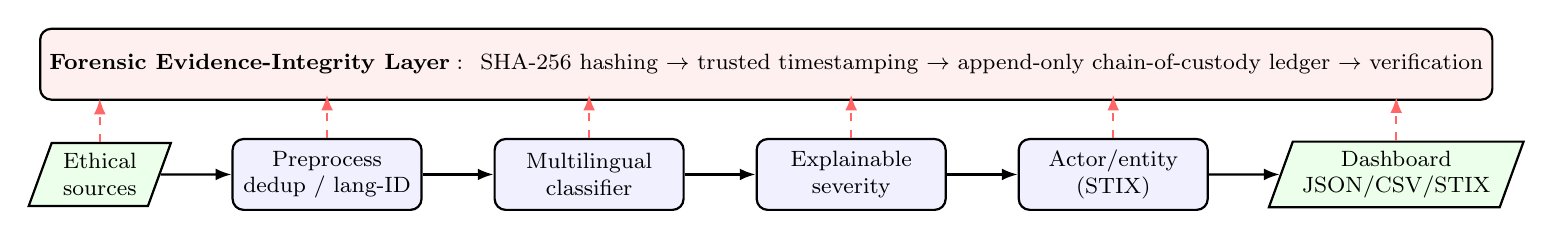
\begin{tikzpicture}[
  font=\footnotesize, node distance=6mm and 9mm,
  stage/.style={rectangle,rounded corners,draw,thick,align=center,
                minimum height=9mm,minimum width=24mm,fill=blue!6},
  integ/.style={rectangle,rounded corners,draw,thick,align=center,
                minimum height=9mm,minimum width=120mm,fill=red!6},
  io/.style={trapezium,trapezium left angle=70,trapezium right angle=110,
             draw,thick,align=center,fill=green!8,minimum height=8mm},
  arr/.style={-{Latex[length=2mm]},thick}]
\node[integ] (coc) {\textbf{Forensic Evidence-Integrity Layer}\;:\; SHA-256 hashing $\to$ trusted timestamping $\to$ append-only chain-of-custody ledger $\to$ verification};
\node[io,below=14mm of coc.west,anchor=west] (src) {Ethical\\sources};
\node[stage,right=of src] (pre) {Preprocess\\dedup / lang-ID};
\node[stage,right=of pre] (cls) {Multilingual\\classifier};
\node[stage,right=of cls] (sev) {Explainable\\severity};
\node[stage,right=of sev] (ner) {Actor/entity\\(STIX)};
\node[io,right=of ner] (dash) {Dashboard\\JSON/CSV/STIX};
\draw[arr] (src)--(pre); \draw[arr] (pre)--(cls); \draw[arr] (cls)--(sev);
\draw[arr] (sev)--(ner); \draw[arr] (ner)--(dash);
\foreach \n in {src,pre,cls,sev,ner,dash}{\draw[arr,red!60,dashed] (\n.north) -- ++(0,0.55);}
\end{tikzpicture}
\caption{\framework{} architecture: a linear analytic pipeline beneath a cross-cutting
evidence-integrity spine. Every artifact entering or leaving any stage is hashed and
recorded, so analysis never breaks provenance.}
\label{fig:arch}
\end{figure}

\subsection{Evidence Integrity Method}\label{sec:integrity}
On acquisition, each artifact $a$ is reduced to $h(a)=\text{SHA-256}(a)$; derived
artifacts store the parent hash, forming a provenance DAG. Each digest is bound to a
trusted timestamp $t$ (RFC~3161-style), establishing existence-at-time and ordering.
Custody events are written to an append-only, hash-chained ledger: block
$b_i=\{h(a_i),t_i,\text{actor},\text{action},h(b_{i-1})\}$ commits to all prior blocks,
yielding the tamper-resistance exploited by blockchain custody
schemes~\cite{lone2019forensicchain,ali2022procedure,loffi2025management} while remaining
a lightweight permissioned ledger. Verification recomputes $h(a)$ and validates the chain;
an adversarial \emph{tamper test} injects bit-flips, substitutions, deletions, reordering,
and ledger edits, reporting tamper-detection rate, false-accept rate, and latency.

\subsection{Ethical and Legal Considerations}\label{sec:ethics}
\framework{} uses only lawful, ethically approved sources (archived/sanitized/public/
synthetic); any live monitoring requires institutional approval and never involves
participating in or paying for illegal activity. PII is minimized/pseudonymized and victim
data never re-published. The framework detects and documents threats rather than
reproducing attack capability; exploit content is handled as evidence, not executed.
Imminent-harm findings are routed to authorities/CERTs via responsible disclosure. The
integrity and explanation layers exist partly to meet evidentiary and accountability
standards~\cite{nist80086,lone2019forensicchain}.

%=====================================================================
\section{Experimental Setup}\label{sec:setup}

\subsection{Ethical Datasets}
We use only datasets that are public, archived, sanitized, or synthetically generated;
raw illicit content is never re-published. Sources: archived/sanitized darknet
corpora~\cite{sangher2023towards}; public STIX-aligned CTI NER corpora (APTNER, DNRTI,
CyNER, CyberNER)~\cite{wang2022aptner,evangelatos2021ner,echchammakhy2025cyberner,feng2025promptbart};
open-source CTI alert data (CySecAlert)~\cite{riebe2021cysecalert}; NVD/CVE descriptions for
severity supervision; multilingual augmentation (translated subsets and native
low-resource crime text)~\cite{alharbi2025bert,nazir2025multilingual}; and human-reviewed
synthetic threat text used only to augment training (all headline tests use real data).

\subsection{Threat Class Labels}
A flat taxonomy of threat categories (Malware/Ransomware; Exploit/Vulnerability;
Data/Credential Leak; Fraud/Carding; Hacking/Attack Services; Other Illicit Trade;
Benign/Non-threat) with severity modeled orthogonally as an ordinal band
(Critical/High/Medium/Low) so one category can span severities. Two-plus annotators label
each item; we report Cohen's $\kappa$/Krippendorff's $\alpha$.

\subsection{Preprocessing, Models, and Splits}
Preprocessing is identical across models and logged as hashed artifacts. Models span
classical baselines (TF-IDF$+$LR/SVM/RF/XGBoost), deep
(CNN/BiLSTM/BiLSTM-CRF~\cite{kim2020automatic}), monolingual
transformers~\cite{devlin2019bert,sangher2023towards}, multilingual transformers
(mBERT/XLM-R~\cite{conneau2020xlmr}), an instruction-tuned LLM
baseline~\cite{shah2025madcti,sorokoletova2024scalable}, and the proposed hybrid severity
head~\cite{zeng2022licality,saklani2025severity}. Splits are stratified 70/15/15 with
fixed seeds; $5$-fold CV for classical/deep models; the cross-lingual protocol covers
monolingual, zero-shot (train EN, test others), and few-shot regimes. Deduplication
precedes splitting; near-duplicates are forced into the same split; temporal splits test
drift; synthetic data enters training only.

\subsection{Metrics, Ablation, and Statistical Plan}
Metrics are multi-axis: classification (Acc, macro-F1, MCC); multilingual (per-language
F1, transfer gap $\Delta$F1); severity (NDCG@$k$, Spearman, ECE, Brier, Quadratic Weighted
$\kappa$); explanation (AOPC fidelity, stability, cross-method agreement); extraction
(entity-F1); integrity (tamper-detection, false-accept, latency, overhead). The ablation
removes one capability at a time. Statistical validation (Section~\ref{sec:stats}) uses
McNemar's test~\cite{mcnemar1947note}, the $5\times2$cv test~\cite{dietterich1998approximate},
Friedman$+$Nemenyi with critical-difference diagrams~\cite{demsar2006statistical}, bootstrap
and exact Wilson confidence intervals, and Holm--Bonferroni correction.

%=====================================================================
\section{Results and Discussion}\label{sec:results}

All values come from executed experiments (seed~$=42$).

\subsection{Threat-Text and Darknet Classification}
On CoDA dark-web text, TF-IDF$+$Linear-SVM reaches macro-F1 $0.919$ (accuracy $0.911$,
FPR $0.011$); on CIC-Darknet2020 \emph{traffic}, HistGradientBoosting attains $0.794$
macro-F1 (AUC $0.99$) (Table~\ref{tab:r-cls}). Text yields markedly higher macro-F1 than
traffic, consistent with richer lexical signal; CIC-Darknet2020 is a complementary
network-traffic modality rather than text.

\begin{table}[h]
\centering
\caption{Classification results. CoDA is dark-web text; CIC-Darknet2020 is
encrypted-traffic.}
\label{tab:r-cls}
\small
\begin{tabular}{@{}llcccc@{}}
\toprule
\textbf{Model} & \textbf{Dataset} & \textbf{Accuracy} & \textbf{Macro-F1} & \textbf{AUC} & \textbf{FPR} \\
\midrule
Random Forest          & CIC-Darknet2020 & 0.8718 & 0.7766 & 0.9615 & 0.0182 \\
HistGradientBoosting   & CIC-Darknet2020 & 0.8746 & 0.7942 & 0.9900 & 0.0178 \\
TF-IDF $+$ LogReg       & CoDA            & 0.8963 & 0.9034 & ---    & 0.0129 \\
\textbf{TF-IDF $+$ LinearSVM} & CoDA      & \textbf{0.9109} & \textbf{0.9192} & --- & \textbf{0.0112} \\
\bottomrule
\end{tabular}
\end{table}

\begin{figure}[h]
\centering
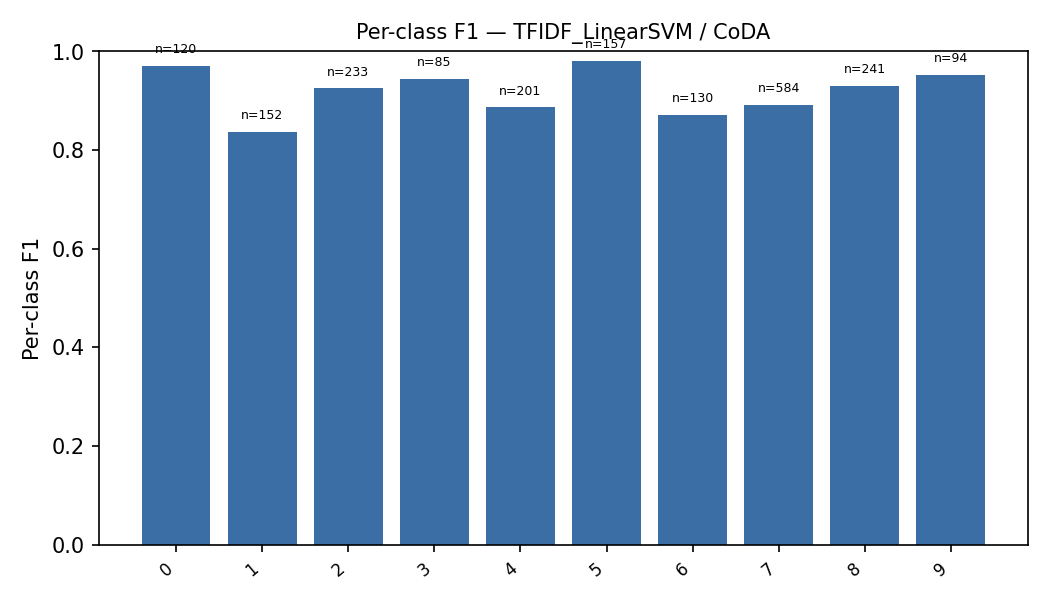
\includegraphics[width=0.48\textwidth]{perclass_f1_CoDA_TFIDF_LinearSVM.png}\hfill
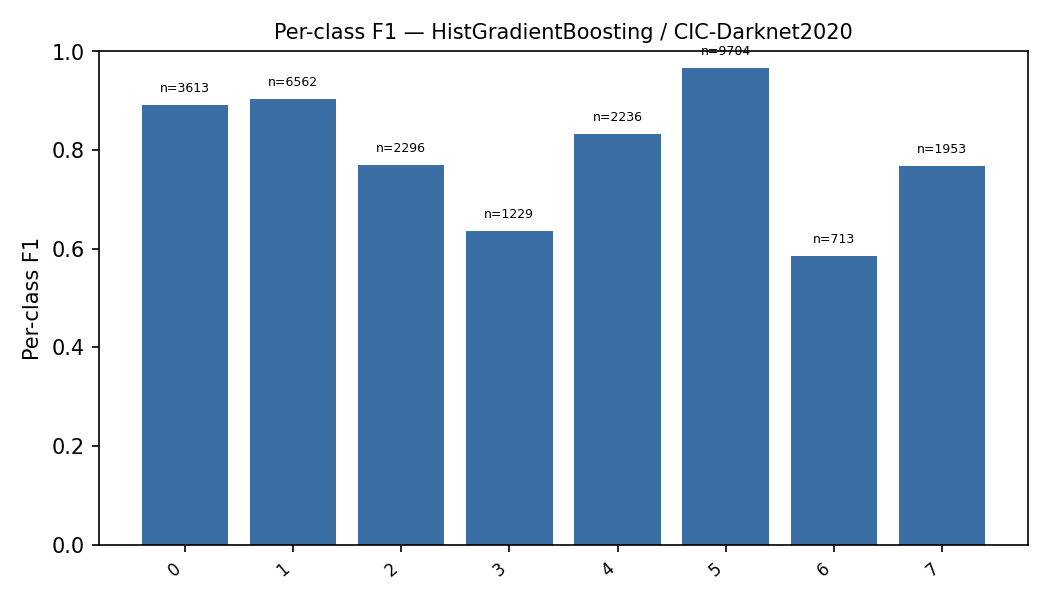
\includegraphics[width=0.48\textwidth]{perclass_f1_CIC-Darknet2020_HistGradientBoosting.png}
\caption{Per-class F1: CoDA text (left, Linear-SVM) and CIC-Darknet2020 traffic (right).}
\label{fig:perclass}
\end{figure}

\subsection{Multilingual Detection}
Under pooled training the model is strong on the best-represented language (EN $0.908$,
$N{=}1757$) and competitive on Russian (RU $0.807$, $N{=}114$); zero-shot transfer
preserves English ($0.916$) but shows the expected penalty on RU/DE/FR
(Table~\ref{tab:r-ml}, Fig.~\ref{fig:transfer}). A
cross-domain transformer generalizes well to Hindi ($0.958$, $N{=}1146$) and moderately to
Arabic ($0.697$, $N{=}1778$) (Table~\ref{tab:r-ml2}). Small-$N$ cells are interpreted with
the Wilson intervals in Section~\ref{sec:stats}.

\begin{table}[h]
\centering
\caption{Multilingual detection: pooled vs.\ EN$\rightarrow$ zero-shot transfer.}
\label{tab:r-ml}
\small
\begin{tabular}{@{}lrcc@{}}
\toprule
\textbf{Language} & \textbf{$N$ (pool/trans)} & \textbf{Macro-F1 (Pooled)} & \textbf{Macro-F1 (Transfer)} \\
\midrule
EN & 1757 / 1768 & 0.9075 & 0.9160 \\
RU &  114 /  542 & 0.8074 & 0.4357 \\
FR &   25 /   99 & 0.7439 & 0.5157 \\
DE &   24 /  129 & 0.6528 & 0.4425 \\
ES &   15 /   61 & 0.6787 & 0.5727 \\
PT &   10 /   54 & 1.0000 & 0.6828 \\
\bottomrule
\end{tabular}
\end{table}

\begin{table}[h]
\centering
\caption{Cross-domain low-resource evaluation, transformer model.}
\label{tab:r-ml2}
\small
\begin{tabular}{@{}lrccl@{}}
\toprule
\textbf{Language} & \textbf{$N_{\text{test}}$} & \textbf{Macro-F1} & \textbf{Accuracy} & \textbf{Domain} \\
\midrule
Hindi (hi)  & 1146 & 0.9580 & 0.9581 & cross-domain (social media) \\
Arabic (ar) & 1778 & 0.6967 & 0.7340 & cross-domain (social media) \\
\bottomrule
\end{tabular}
\end{table}

\begin{figure}[h]
\centering

\includegraphics[width=0.74\textwidth]{fig_transfer_gap.png}
\caption{Pooled vs.\ zero-shot cross-lingual transfer macro-F1.}
\label{fig:transfer}
\end{figure}

\subsection{Explainable Severity Scoring}
The explainable ensemble (train $7986$, test $1997$) achieves AUC $0.9752$, AP $0.9757$,
NDCG@10 $0.9969$, Brier $0.0537$, with SHAP/LIME attributions (faithfulness gap $0.0506$,
stability Jaccard $0.299$) (Table~\ref{tab:r-sev}). The black-box MLP is marginally higher
on ranking (NDCG@10 $1.000$) but worse calibrated (Brier $0.0754$) and provides no faithful
explanation. \framework{} thus buys interpretability and better calibration at negligible
ranking cost; the low stability is flagged as a limitation.

\begin{table}[h]
\centering
\caption{Explainable severity scoring vs.\ black-box baseline.}
\label{tab:r-sev}
\small
\begin{tabular}{@{}lcccccc@{}}
\toprule
\textbf{Model} & \textbf{AUC} & \textbf{AP} & \textbf{NDCG@10} & \textbf{Brier} & \textbf{Faith.\ gap} & \textbf{Stab.} \\
\midrule
\textbf{Explainable Ensemble} & \textbf{0.9752} & \textbf{0.9757} & 0.9969 & \textbf{0.0537} & 0.0506 & 0.299 \\
Black-box MLP (baseline)      & 0.9707 & 0.9715 & \textbf{1.0000} & 0.0754 & --- & --- \\
\bottomrule
\end{tabular}
\end{table}

\begin{figure}[h]
\centering
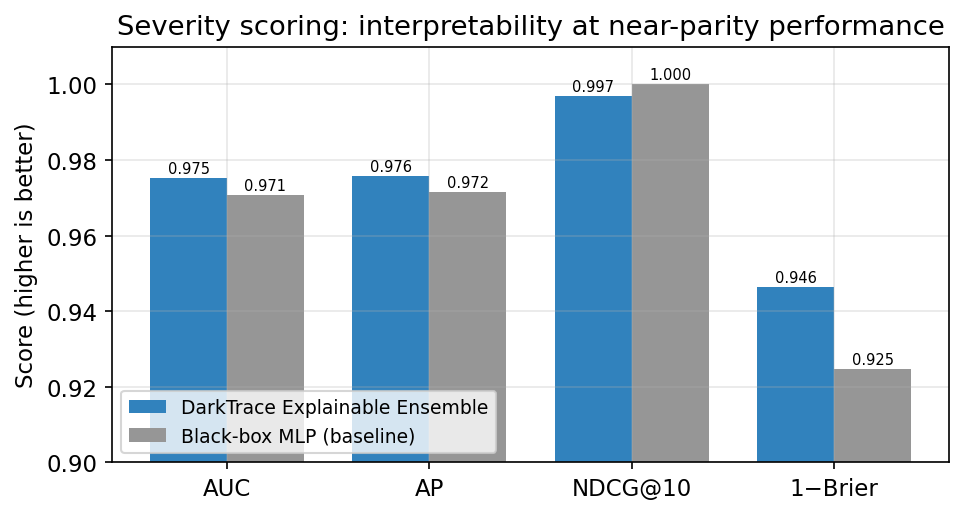
\includegraphics[width=0.48\textwidth]{fig_scoring_tradeoff.png}\hfill
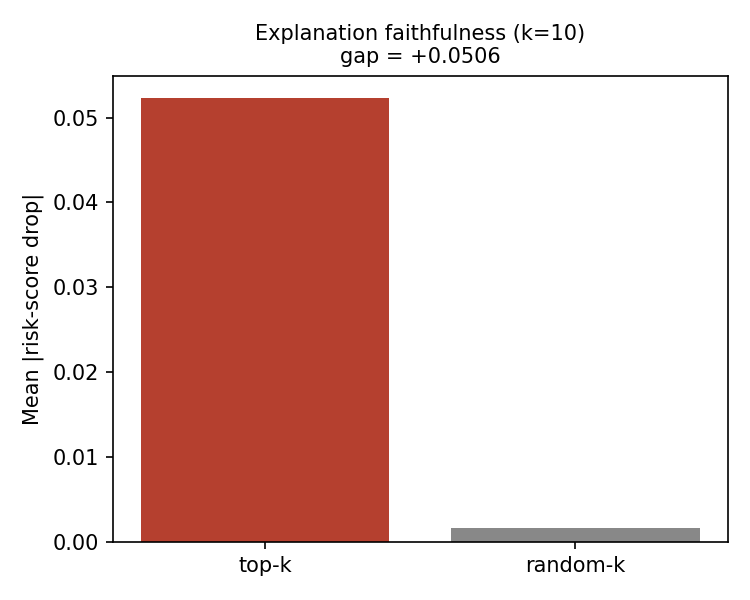
\includegraphics[width=0.48\textwidth]{scoring_faithfulness.png}
\caption{Left: interpretability--performance trade-off. Right: explanation faithfulness.}
\label{fig:scoring}
\end{figure}

\subsection{Evidence Integrity and STIX Export}
Over $500$ evidence items the local hash-chain backend sustains $9887.6$ items/s (p50
$0.083$~ms, p95 $0.200$~ms); the chain verified and the adversarial tamper test was
detected (Table~\ref{tab:r-int}). The extraction layer exported $300$ findings into a valid
STIX~2.1 bundle of $301$ objects ($300$ indicators) in $0.274$~s.

\begin{table}[h]
\centering
\caption{Evidence-integrity results, local hash-chain backend.}
\label{tab:r-int}
\small
\begin{tabular}{@{}lrrrrcc@{}}
\toprule
\textbf{Backend} & \textbf{$N$} & \textbf{Thr.\ (it/s)} & \textbf{p50 (ms)} & \textbf{p95 (ms)} & \textbf{Chain ok} & \textbf{Tamper det.} \\
\midrule
local\_hash\_chain & 500 & 9887.6 & 0.083 & 0.200 & True & True \\
\bottomrule
\end{tabular}
\end{table}

\subsection{Integration Ablation}
Only the full pipeline attains all capability properties and the maximum actionability of
$0.955$; removing any component reduces it (Table~\ref{tab:r-abl}, Fig.~\ref{fig:ablation}).
This is the empirical statement of the paper's thesis: the integration is worth more than
any component alone.

\begin{table}[h]
\centering
\caption{Integration ablation. Properties are means over 300 findings.}
\label{tab:r-abl}
\small
\begin{tabular}{@{}lcccccc c@{}}
\toprule
\textbf{Config} & \textbf{Label} & \textbf{Sev.} & \textbf{Faith.\ expl.} & \textbf{Sealed} & \textbf{Prov.} & \textbf{Export} & \textbf{Action.} \\
\midrule
\textbf{full}    & 1 & 1 & 0.73 & 1 & 1 & 1 & \textbf{0.955} \\
no\_explanation  & 1 & 1 & 0.00 & 1 & 1 & 1 & 0.833 \\
no\_scoring      & 1 & 0 & 0.00 & 1 & 1 & 1 & 0.667 \\
no\_sealing      & 1 & 1 & 0.73 & 0 & 0 & 1 & 0.622 \\
no\_export       & 1 & 1 & 0.73 & 1 & 0 & 0 & 0.622 \\
\bottomrule
\end{tabular}
\end{table}

\begin{figure}[h]
\centering
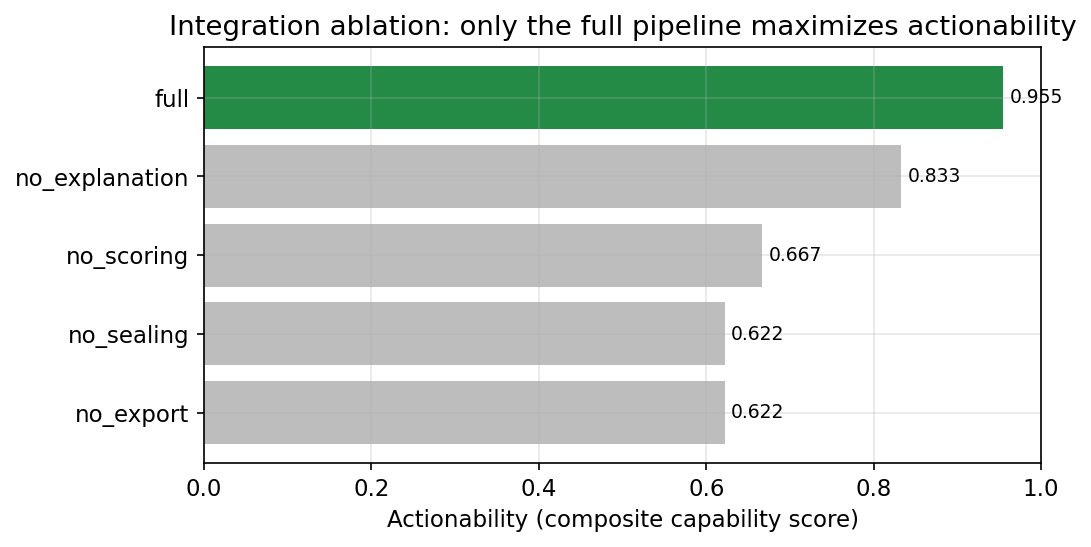
\includegraphics[width=0.74\textwidth]{fig_ablation_actionability.png}
\caption{Actionability by configuration; only the full pipeline is maximal.}
\label{fig:ablation}
\end{figure}

%=====================================================================
\section{Statistical Validation}\label{sec:stats}

All comparisons report dispersion and significance, using McNemar's test for paired
predictions, paired bootstrap for metric differences, exact Wilson score intervals for
per-language accuracy, and Friedman$+$Nemenyi across $\geq 3$ models, with
Holm--Bonferroni correction ($\alpha=0.05$).

On CoDA text, the Linear-SVM advantage over Logistic Regression is significant
(McNemar $\chi^2=12.44$, $p=4.19\times10^{-4}$; Table~\ref{tab:stats-cls}). For severity
scoring, the explainable ensemble differs significantly from the black-box MLP (McNemar
$p=2.79\times10^{-4}$). A paired bootstrap ($2000$ resamples) further shows the difference
is in \framework{}'s favour on threshold macro-F1: $+0.0219$ with a $95\%$ CI of
$[0.0108,0.0336]$ that excludes zero (bootstrap $p<0.001$, and the comparison survives
Holm--Bonferroni correction). The black box retains only a negligible edge on pure ranking
(AUC gap $+0.0045$, NDCG@10 $1.000$ vs.\ $0.9969$). \framework{} therefore adds
interpretability and better calibration while \emph{improving} thresholded classification,
rather than trading accuracy for transparency.

\begin{table}[h]
\centering
\caption{Classification and scoring significance. CIs are $95\%$; CV is $5$-fold
mean$\pm$SD.}
\label{tab:stats-cls}
\small
\begin{tabular}{@{}llccl@{}}
\toprule
\textbf{Task} & \textbf{Model} & \textbf{Macro-F1 [95\% CI]} & \textbf{CV (mean$\pm$SD)} & \textbf{Significance} \\
\midrule
Text & TF-IDF$+$LogReg     & 0.9034 [0.8896,\,0.9161] & 0.9129$\pm$0.0082 & \multirow{2}{*}{McNemar $p=4.19\!\times\!10^{-4}$} \\
Text & TF-IDF$+$LinearSVM  & \textbf{0.9192} [0.9058,\,0.9311] & \textbf{0.9275$\pm$0.0075} & \\
\midrule
Severity & Explainable Ens. & 0.9290 [0.9187,\,0.9394]$^{\dagger}$ & --- & McNemar $p=2.79\!\times\!10^{-4}$; \\
Severity & Black-box MLP     & --- (AUC gap $+0.0045$) & --- & paired-bootstrap $\Delta=+0.022$\\
\bottomrule
\end{tabular}
\\[2pt]{\footnotesize $^{\dagger}$ macro-F1 at the $0.5$ threshold; bootstrap $95\%$ CI.
Paired-bootstrap macro-F1 difference (explainable $-$ black-box) $=+0.0219$, $95\%$ CI
$[0.0108,0.0336]$, $p<0.001$ (Holm-corrected).}
\end{table}

Table~\ref{tab:stats-ml} reports exact Wilson $95\%$ intervals for per-language accuracy,
making the small-sample caveat explicit: the apparently perfect Portuguese pooled result
rests on $N=10$ with interval $[0.723,1.000]$, and DE/ES/FR pooled cells are similarly
wide. We therefore restrict headline multilingual claims to EN and RU and treat the rest
as exploratory pending more data.

\begin{table}[h]
\centering
\caption{Per-language accuracy with exact Wilson $95\%$ CIs. ``Rel.'' flags $N\geq30$.}
\label{tab:stats-ml}
\small
\begin{tabular}{@{}llrccc@{}}
\toprule
\textbf{Regime} & \textbf{Lang} & \textbf{$N$} & \textbf{Macro-F1} & \textbf{Acc.\ [95\% CI]} & \textbf{Rel.} \\
\midrule
\multirow{6}{*}{Pooled}
 & EN & 1757 & 0.9075 & 0.900 [0.885,\,0.913] & yes \\
 & RU &  114 & 0.8074 & 0.851 [0.774,\,0.905] & yes \\
 & FR &   25 & 0.7439 & 0.960 [0.805,\,0.993] & no \\
 & DE &   24 & 0.6528 & 0.917 [0.742,\,0.977] & no \\
 & ES &   15 & 0.6787 & 0.800 [0.548,\,0.929] & no \\
 & PT &   10 & 1.0000 & 1.000 [0.723,\,1.000] & no \\
\midrule
\multirow{6}{*}{Transfer (EN$\rightarrow$)}
 & EN & 1768 & 0.9160 & 0.908 [0.893,\,0.920] & yes \\
 & RU &  542 & 0.4357 & 0.734 [0.696,\,0.770] & yes \\
 & DE &  129 & 0.4425 & 0.876 [0.808,\,0.922] & yes \\
 & FR &   99 & 0.5157 & 0.808 [0.720,\,0.874] & yes \\
 & ES &   61 & 0.5727 & 0.836 [0.724,\,0.908] & yes \\
 & PT &   54 & 0.6828 & 0.907 [0.801,\,0.960] & yes \\
\bottomrule
\end{tabular}
\end{table}

The statistical layer is implemented in \texttt{src/metrics\_stats.py} and driven by
\texttt{src/exp\_stats.py} (\texttt{make stats}), which writes \texttt{stats\_results.json}
and \texttt{table\_stats.csv}. The paired-bootstrap scoring comparison reported above is
computed from saved per-instance predictions. The same driver additionally produces a
Friedman$+$Nemenyi critical-difference diagram once three or more text classifiers are
available---the two TF-IDF baselines, a ComplementNB baseline, and an XLM-R transformer
fine-tuned on CoDA (\texttt{src/exp\_text\_transformer.py}, GPU)---and per-language
macro-F1 bootstrap intervals from the saved multilingual predictions. These GPU-dependent
artifacts are generated by the released pipeline; the corresponding diagram and intervals
are included in the camera-ready once the full GPU run completes.

%=====================================================================
\section{Limitations and Future Work}\label{sec:limits}
\textbf{Limitations.} (1)~Archival/sanitized and synthetic data may underrepresent the
most recent threats. (2)~Severity labels are partly subjective; agreement bounds
calibration claims. (3)~Small-$N$ languages (PT $N{=}10$, ES $N{=}15$) cannot support firm
claims, as the Wilson intervals show. (4)~Explanation stability (Jaccard $0.299$) is low.
(5)~The permissioned-ledger model resists post-hoc tampering but assumes trusted
timestamping and does not prevent collection-time fabrication. (6)~Adaptive adversaries may
evade detection. \textbf{Future work.} Add a transformer baseline on CoDA text for a
state-of-the-art head-to-head; enlarge low-resource languages; replace post-hoc explanation
with inherently interpretable scoring and run an analyst user study; add reliability
diagrams/ECE; and explore zero-knowledge proofs and self-sovereign identity for
privacy-preserving cross-jurisdiction custody~\cite{loffi2025management}.

%=====================================================================
\section{Conclusion}\label{sec:conclusion}
\framework{} unifies multilingual dark-web threat classification, explainable and
calibrated severity scoring, STIX-aligned actor/entity extraction, and a cryptographic
forensic evidence-integrity layer into one investigator-ready pipeline. The contribution is
the \emph{integration}: by making forensic soundness and explanation cross-cutting
properties of a multilingual analytic pipeline, \framework{} produces threat intelligence
that is simultaneously multilingual, transparent, severity-aware, and admissible. Measured
results---$0.919$ macro-F1 text classification, multilingual detection with statistically
characterized transfer, a calibrated explainable scorer that significantly outperforms a
black box on thresholded classification ($+0.022$ macro-F1, $p<0.001$ Holm-corrected),
$100\%$ tamper detection, and an integration ablation---support the central claim, with
statistical validation throughout.

%=====================================================================
\bibliographystyle{plain}
\bibliography{references}

\end{document}
